\section{Lecture 5. PageRank}
\begin{multicols}{2}
\subsection{PageRank Model}
\subsubsection{Importance score}
\begin{itemize}
    \item [-] $v_i$: importance score of page $i$
    \item [-] $c_j$: number of outgoing links of page $j$
    \item [-] $\mathcal{L}_i$: set of pages that refers to page $i$
\end{itemize}
\[
    \begin{array}{c}
        v_i = |\mathcal{L}_i| \\
        \Downarrow \\
        v_i = \sum_{j\in \mathcal{L}_i} v_j \\
        \Downarrow \\
        v_i = \sum_{j\in \mathcal{L}_i} \frac{v_j}{c_j}
    \end{array}
\]
\subsubsection{The model}
e.g. \\
\centerline{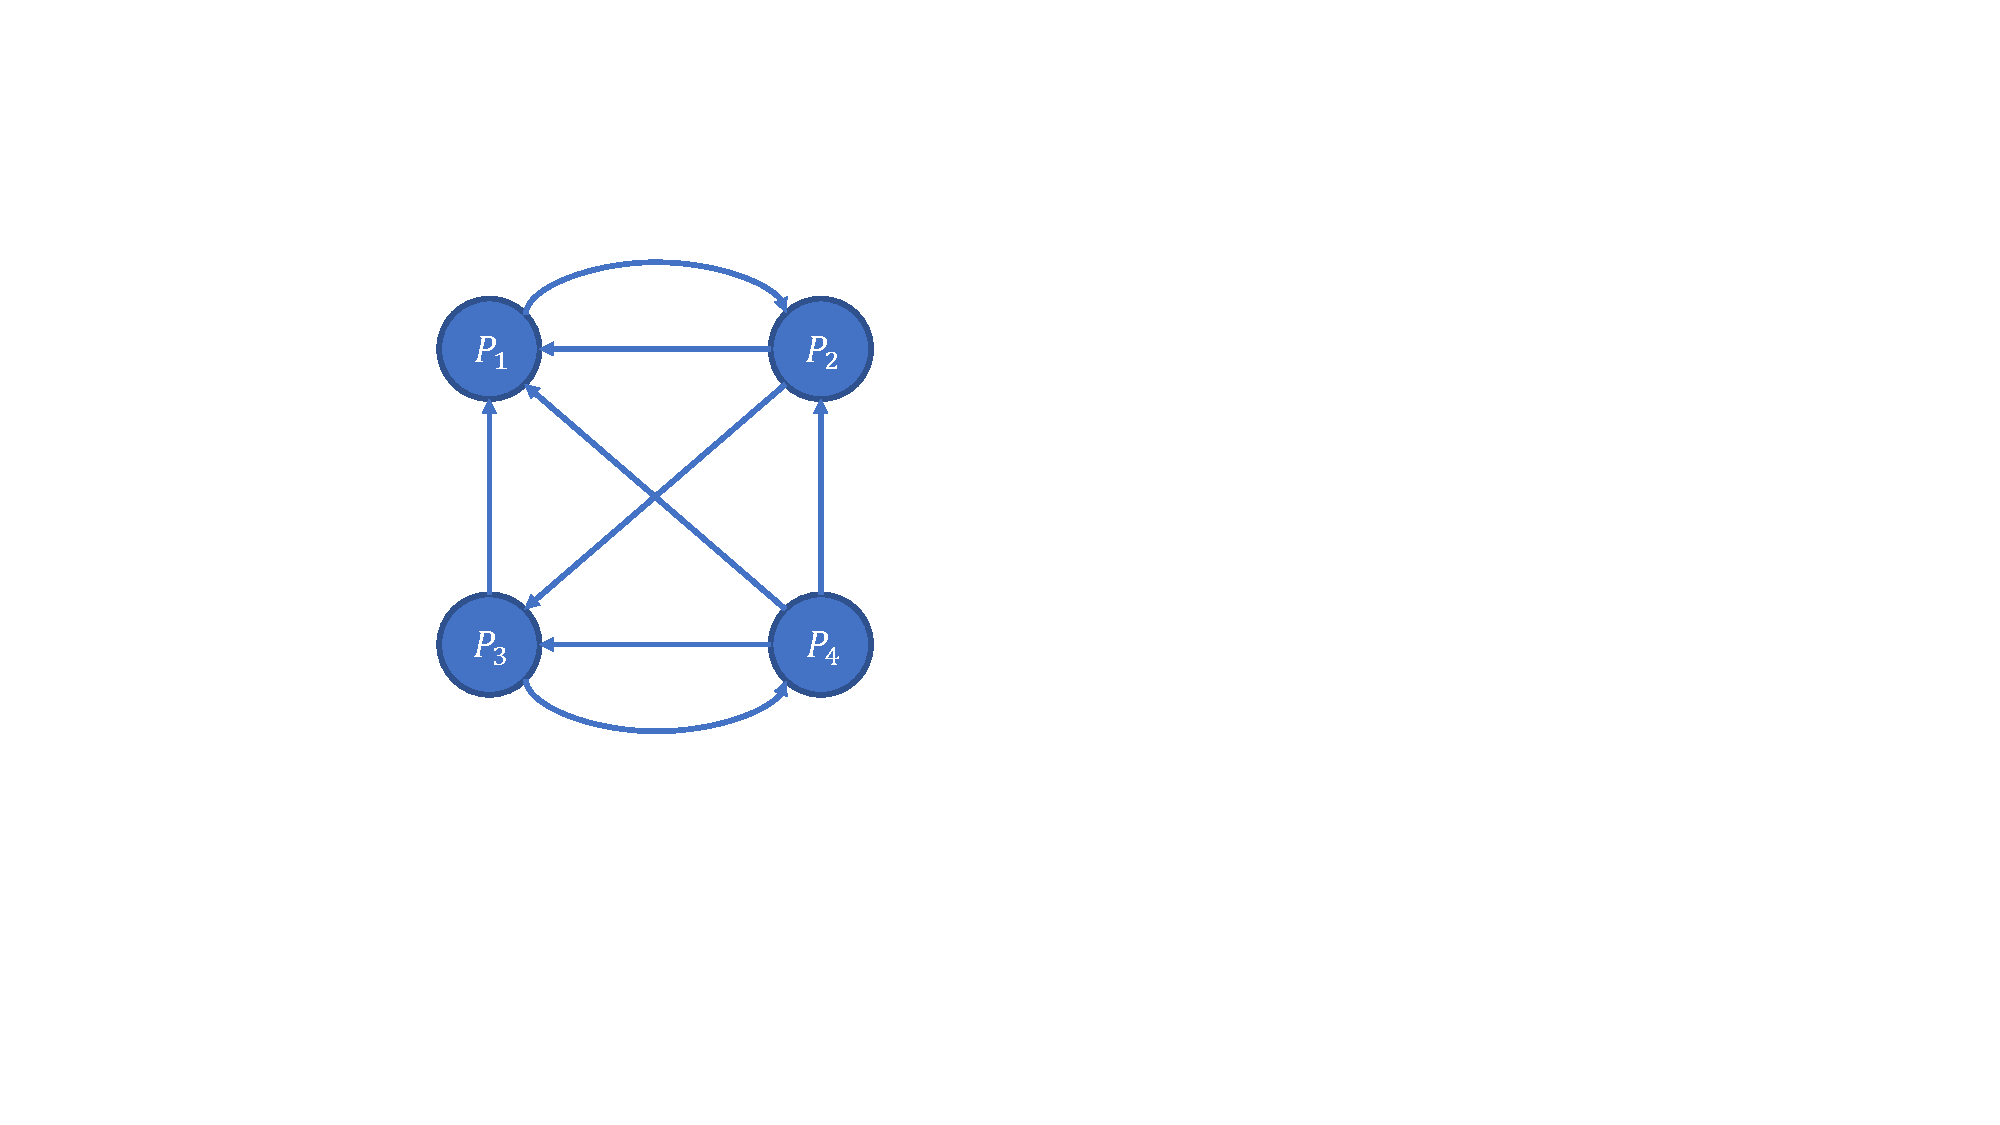
\includegraphics[width=5cm]{sections/lecture_5_fig1.pdf}} \\
$v_1 = 1\cdot v_2 + \frac{1}{2}v_3 + \frac{1}{3}v_4$ \\
$v_2 = 1\cdot v_1 + \frac{1}{3}v_4$ \\
... \\
$\Longrightarrow$
\[
    \underbrace{
    \begin{bmatrix}
        0  &  1/2  &  1/2  &  1/3  \\
        1  &  0    &  0    &  1/3  \\
        0  &  1/2  &  0    &  1/3  \\
        0  &  0    &  1/2  &  0    \\
    \end{bmatrix}
    }_{\text{\rm link matrix}}
    \begin{bmatrix}
        v_1 \\ v_2 \\ v_3 \\ v_4
    \end{bmatrix}
    =
    \begin{bmatrix}
        v_1 \\ v_2 \\ v_3 \\ v_4
    \end{bmatrix}
\]
$\Longrightarrow$
\[
    Av = v\quad ,\quad v \geq 0
\]

\subsection{PageRank Problem}
Find solution $v\geq 0$ satisfying $Av=v$ \\
The foure questions:
\begin{enumerate}
    \item Does $A$ admit a solution of $Av=v$?          \\ (Does $A$ has eigenvalue equal to 1?)
    \item Does $Av=v$ admit a non-negative solution?    \\ ($v\geq 0$ or $v\leq 0$)
    \item Is the solution unique?                       \\ (unique ranking)
    \item Can we obtain the solution efficiently?       \\ (Power method applicable?)
\end{enumerate}

\subsubsection{Answer to Question 1}
Does $A$ admit a solution of $Av=v$? (Does $A$ has eigenvalue equal to 1?)

Note that $A\geq 0$ and column-sum eqaul to 1 (column-stochastic matrix). \\
$\Longrightarrow$ $\textbf{1}^TA=\textbf{1}^T$ \\
$\Longrightarrow$ $A^T\cdot \textbf{1} = \textbf{1}$ \\
$\Longrightarrow$ $A^T$ has an eigenvalue equal to 1 \\
Since $A$ and $A^T$ have the same set of eigenvalues \\
$\Longrightarrow$ $A$ has an eigenvlue equal to 1 \\

\begin{theorem}
    Let $A$ be non-negative and column(row)-stochastic, then
    \begin{enumerate}
        \item $\lambda=1$ is an eigenvlue of $A$
        \item $|\lambda|\leq 1$ for all eigenvalues of $A$
    \end{enumerate}
\end{theorem}
\begin{proof}
    Let $Av = \lambda v$ for some $|\lambda|\neq 1$. \\
    Let $|v_k| = \max \{|v_1|,|v_2|,...,|v_m|\}$.
    \[
        \lambda v_k = \sum_{i=1}^m [A]_{ki}v_i
    \]
    $\Longrightarrow$
    \[
        \begin{array}{ll}
            |\lambda||v_k|  &= |\sum_{i=1}^m[A]_{ki}v_i| \\
                            &\leq \sum_{i=1}^m|[A]_{ki}|\cdot |v_i| \\
                            &\leq |v_k|\cdot \sum_{i=1}^m|[A]_{ki}| \\
                            &= |v_k|
        \end{array}
    \]
    $\Longrightarrow$
    \[
        |\lambda|\leq 1
    \]
\end{proof}

\textbf{Disjoint page networks}
\[
    A = \begin{bmatrix}
        A_1 & 0 \\ 0 & A_2
    \end{bmatrix}
\]
\[
    \begin{array}{l}
        A_1 v_1 = v_1 \\ A_2 v_2 = v_2
    \end{array}
\]
\[
    A
    \left( \alpha_1 \left(\begin{array}{c} v_1 \\ 0 \end{array}\right) + \alpha_2 \left(\begin{array}{c} v_1 \\ 0 \end{array}\right) \right) 
    = 
    \left( \alpha_1 \left(\begin{array}{c} v_1 \\ 0 \end{array}\right) + \alpha_2 \left(\begin{array}{c} v_1 \\ 0 \end{array}\right) \right) 
\]

\textbf{Modified model}
\[
    M \triangleq (1-\beta) A + \beta \left( \frac{11^T}{m} \right) > 0
\]
This is positive column-stochastic
\[
    1^TM = (1-\beta)1^TA + \beta 1^T \left( \frac{11^T}{m} \right) = 1^T
\]

\subsubsection{Answer to Question 2}
Does $Av=v$ admit a non-negative solution? ($v\geq 0$ or $v\leq 0$)

\begin{theorem}
    For positive and column-stochastic matrix $M$, any eigenvector associated with $\lambda_1$ has either all positive or all negative components.
\end{theorem}
\begin{proof}
    Note that for $y\in\mathbb{R}^m$, $|\sum_{i=1}^m y_i| < \sum_{i=1}^m |y_i|$ if $\{y_i\}$ have mixed signs. \\
    Suppose the above theorem is not true. Then we have
    \[
        |v_i| = |\sum_{j=1}^m [M]_{ij}v_j| < \sum_{j=1}^m [M]_{ij}|v_j|
    \]
    $\Longrightarrow$
    \[
        \sum_{i=1}^m |v_i| < \sum_{i=1}^m \sum_{j=1}^m [M]_{ij}v_j = \sum_{j=1}^m\sum_{i=1}^m  [M]_{ij}v_j = \sum_{j=1}^m |v_j|
    \]
    Contradict! So the above theorem is true.
\end{proof}

\subsubsection{Answer to Question 3}
Is the solution unique? (unique ranking) \\
Since $Mv=v$ $\Longrightarrow$ $(M-I)v=0$, show 
\[
    dim(Null(M-I))=1
\]
i.e., there is a unique ranking.

\begin{proof}

    Simple lemma: Let $a$ and $b$ be linearly independent, then $\exists x\in span\{a,b\}$ which has mixed sign. \\
    \emph{Proof for this lemma}: \\
    If $1^Tq=0$ $\Longrightarrow$ $q$ has mixed sign. \\
    If $1^Tq\neq 0$, set $\alpha_1 = \frac{-1^Tb}{1^Tq}$, $\alpha_2=1$ and let $x=\alpha_1\cdot a+\alpha_2\cdot b$ \\
    $\Longrightarrow$ $x$ satisfies $1^Tx=0$, so $x$ has mixed sign.

    Suppose $dim(Null(M-I))>1$, then for $q_1,q_2\in Null(M-I)$ that are linear independent.
    $\Longrightarrow$ $\exists v= \alpha_1 q_1  + \alpha_2 q_2 \in Null(M-I)$ \\
    $\Longrightarrow$ $Mv=v$ which has mixed sign. (Contradict!) \\
    $\Longrightarrow$ $dim(Null(M-I))=1$
\end{proof}

\subsubsection{Answer to Question 4}
Can we obtain the solution efficiently? (Power method applicable?) \\
Property:
Let $M$ be positive and column-stochastic. \\
Let $S=\{v\in \mathbb{R}^m | 1^Tv=0 \}$. \\
Then,
\begin{enumerate}
    \item $Mv\in S$ if $v\in S$
    \item $\|Mv\|_1 \leq c\|v\|_1$ with $c<1$ $\forall$ any $v\in S$
    \item the eigenvector associated with $\lambda=1$, denoted $v_1$, can be obtainable by the power method
\end{enumerate}
\begin{proof} \\
    1) \\
    $v\in S$ $\Longleftrightarrow$ $1^Tv=0$ \\
    2) \\
    $w\triangleq Mv$ \\
    $\begin{array}{ll}
        \|w\|_1 &= \|Mv\|_1 \\
                &= \sum_{i=1}^m |w_i| = \sum_{i=1}^m sign(w_i)\cdot w_i \\
                &= \sum_{i=1}^m \left[ sign(w_i)\cdot \sum_{j=1}^m M_{ij}v_j \right] \\
                &= \sum_{j=1}^m \left[ \left( \sum_{j=1}^m sign(w_i)M_{ij} \right) \cdot v_j \right]
    \end{array}$\\
    $a_j\triangleq \left( \sum_{j=1}^m sign(w_i)M_{ij} \right)$\\
    $\begin{array}{ll}
        |a_j|   &= \left| \sum_{j=1}^m sign(w_i)M_{ij} \right| \\
                &< \sum_{j=1}^m \left| sign(w_i)M_{ij} \right| \\
                &= \sum_{j=1}^m M_{ij} = 1
    \end{array}$\\
    $c\triangleq \max_{j=1,...,m} |a_j| < 1$\\
    $\begin{array}{ll}
        \|Mv\_1| = \|w\|_1  &= \sum_{j=1}^m a_jv_j \\
                            &\leq \sum_{j=1}^m |a_j||v_j| \\
                            &\leq c \sum_{j=1}^m |v_j| \\
                            &= c\cdot \|v\|_1
    \end{array}$\\
    $\Longrightarrow$ $\|Mv\|_1 \leq c\|v\|_1 $ $\forall v\in S$
\end{proof}
\newpage
\end{multicols}